\documentclass[12pt,twoside,letterpaper]{memoir}

\usepackage{import}
%% GENERAL ADD ONS %%%%%%%%%%%%%%%%%%%%%%%%%%%%%%%%%%%%%%%%%%%%%%%%%%%%%%%%%%%%

\usepackage[dvipsnames]{xcolor}  %% Must come before Tikz etc.
\usepackage[many]{tcolorbox}
\usepackage{dcounter}
\usepackage{enumerate}
\usepackage{graphicx}
\usepackage[
    hyperindex=true,
    colorlinks=true,
    linkcolor=teal,
    citecolor=ForestGreen]{hyperref}
\usepackage{float}     %% given captions to listings and types.
\usepackage{caption}
\usepackage{subcaption}
% \usepackage{aeguill}  %% IF NEEDED INCLUDE IN Content.tex near top
\usepackage[light]{kpfonts} % Nice Adobe Font
\usepackage{pifont} % \xmark
    \newcommand{\cmark}{\ding{51}}%
    \newcommand{\xmark}{\ding{55}}%

%% TIKZ %%%%%%%%%%%%%%%%%%%%%%%%%%%%%%%%%%%%%%%%%%%%%%%%%%%%%%%%%%%%%%%%%%%%%%%
\usepackage{tikz}
\usepackage{tikz-cd}
    \usetikzlibrary{positioning,arrows,backgrounds}
%%%%%%%%%%%%%%%%%%%%%%%%%%%%%%%%%%%%%%%%%%%%%%%%%%%%%%%%%%%%%%%%%%%%%%%%%%%%%%%

%% MATH %%%%%%%%%%%%%%%%%%%%%%%%%%%%%%%%%%%%%%%%%%%%%%%%%%%%%%%%%%%%%%%%%%%%%%%

\usepackage{amsmath,amsthm,amssymb}

\newcommand{\bigforall}{\mbox{\Large $\mathsurround0pt\forall$}}
\newcommand{\bigexists}{\mbox{\Large $\mathsurround0pt\exists$}}


\usepackage{bussproofs}  %% proof diagrams
\usepackage{wasysym} % \Leftcircle
\usepackage{mathtools}  % left/right harpoons
% \usepackage{lscape}  %% Landscape pages.
% \usepackage{longtable}  %% tables that span 2 pages

%%%%%%%%%%%%%%%%%%%%%%%%%%%%%%%%%%%%%%%%%%%%%%%%%%%%%%%%%%%%%%%%%%%%%%%%%%%%%%%

\usepackage{pdfpages}
% \usepackage{zref-abspos} % Used to know where digress/focus starts/ends

%% STYLE CHAPTERS %%%%%%%%%%%%%%%%%%%%%%%%%%%%%%%%%%%%%%%%%%%%%%%%%%%%%%%%%%%%%
\makechapterstyle{invhangnum}{%
  \setlength\beforechapskip{0pt}%
  \renewcommand*\chapterheadstart{\vspace{\beforechapskip}}%
  \setlength\afterchapskip{2\onelineskip plus .2\onelineskip minus 0.2\onelineskip}%  
  \renewcommand\chaptitlefont{\Huge\bfseries}
  \setlength\midchapskip{-\baselineskip}%
  \renewcommand\chapnumfont{\Huge\bfseries}
  \renewcommand*{\printchaptername}{}
  \renewcommand*{\chapternamenum}{}
  \renewcommand*{\printchapternum}{%
      \raisebox{\dimexpr\midchapskip+\baselineskip\relax}[0pt][0pt]{%
        \makebox[0pt][l]{%
        \makebox[\dimexpr\textwidth+4em\relax][l]{%
          \parbox[t]{\textwidth}{\mbox{}}%
          \parbox[t]{4em}{\hfill\chapnumfont \thechapter}}}}}%
  \renewcommand*{\printchaptertitle}[1]{%
    \raisebox{\dimexpr\midchapskip+\baselineskip\relax}[0pt][0pt]{%
      \parbox[t]{\textwidth}{\raggedright\chaptitlefont ##1}}}%
}
\chapterstyle{invhangnum}
\newlength{\digresslen}
% \chapterstyle{hangnum}
% \hangsecnum

    \usepackage{eso-pic}   %% Used to add gray strip to side of pages.
    %%%%%%%%% Digression margins.
    % \newenvironment{}{}{}
    \newcommand{\digresshere}[1]{
        % \newdimen\digheight
        % \setbox0=\vbox{#1}
        % \digheight=\ht0 \advance\digheight by \dp0
        % \zsavepos{#1-digress}
        % \write\mywrite{#1: \zposy{#1-digress}}%
        % \AddToShipoutPictureBG{%
        % \AtPageLowerLeft{%
        
            % \ifodd\value{page}
            % \hspace*{\dimexpr\paperwidth-3em}%
            % \fi
            % \settoheight{\digresslen}{\vbox{#1}}
        \marginpar{\hspace{\marginparwidth}\textcolor{black!25}{\rule{3em}{1in}}}%
        % }%
        % }%
        % \newcommand{\focus}{\ClearShipoutPictureBG}
    }

    \newcommand{\digress}{
        % \zsavepos{#1-digress}
        % \write\mywrite{#1: \zposy{#1-digress}}%
    \AddToShipoutPictureBG{%
        \AtPageLowerLeft{%
        %\raisebox{.25\paperheight}{%
            \ifodd\value{page}
            \hspace*{\dimexpr\paperwidth-3em}%
            \fi
            \textcolor{black!25}{\rule{3em}{\paperheight}}%
        %}%
        }%
        }
    }
    \newcommand{\focus}{\ClearShipoutPictureBG}
    \newcommand{\codemargin}[1]{
        \marginpar{
            \colorbox{black!25}{
                \parbox{0.9\marginparwidth}{
                    {\small \textsf{#1}}
                }
            }
        }
    }
    %% TOC Formatting
    % Indentation of numbers
    \setlength{\cftsectionindent}{2em}      % default 1.5em

    % Distance between numbers and titles
    \setlength{\cftpartnumwidth}{2.25em}      % default 1.5em
    \setlength{\cftchapternumwidth}{2em}      % default 1.5em
    \setlength{\cftsectionnumwidth}{3em}      % default 2.3em





\usepackage{imakeidx}
    \makeindex
    \indexsetup{headers={Index}{Index}} % Left/Right headers for the index

    \newcommand{\term}[1]{\emph{#1}}%\index{#1}}
%%%%%%%%%%%%%%%%%%%%%%%%%%%%%%%%%%%%%%%%%%%%%%%%%%%%%%%%%%%%%%%%%%%%%%%%%%%%%%%

%% TITLE PAGE %%%%%%%%%%%%%%%%%%%%%%%%%%%%%%%%%%%%%%%%%%%%%%%%%%%%%%%%%%%%%%%%%
\usepackage{epigraph}
\usepackage{titling}
\usepackage{bookman}
    \renewcommand\epigraphflush{flushright}
    \renewcommand\epigraphsize{\normalsize}
    \setlength\epigraphwidth{0.7\textwidth}

    % CSU Green 92, 18, 94, 61
    \definecolor{titlepagecolor}{cmyk}{.92,.18,.94,.61}
    % CSU Gold 11, 6, 64, 13
    \definecolor{titlepagecolor2}{cmyk}{.11,.06,.64,.13}
    %\definecolor{titlepagecolor}{cmyk}{1,.60,0,.40}

    \DeclareFixedFont{\titlefont}{T1}{ppl}{b}{it}{0.5in}
    % The following code is borrowed from: https://tex.stackexchange.com/a/86310/10898

    %%% STOLEN FROM 
    %%%% https://tex.stackexchange.com/questions/85904/showcase-of-beautiful-title-page-done-in-tex
    \newcommand\titlepagedecoration{%
    \begin{tikzpicture}[remember picture,overlay]%,shorten >= -10pt]
    \coordinate (aux1) at ([yshift=-15pt]current page.north east);
    \coordinate (aux2) at ([yshift=-410pt]current page.north east);
    \coordinate (aux3) at ([xshift=8cm, yshift=15cm]current page.south west);
    \coordinate (aux4) at ([yshift=-150pt]current page.north east);

    \node at (aux3) {\begin{tikzpicture}
        \node (e) at (0,0) {$\epsilon$};
        \node (a) at (0:1) {a};
        \node (b) at (120:1) {b};
        \node (c) at (240:1) {c};
        \node (aa) at (-40:2) {aa};
        \node (ba) at (0:2) {ba};
        \node (ca) at (40:2) {ca};
        \node (ab) at (80:2) {ab};
        \node (bb) at (120:2) {bb};
        \node (cb) at (160:2) {cb};
        \node (ac) at (200:2) {ac};
        \node (bc) at (240:2) {bc};
        \node (cc) at (280:2) {cc};
    
        \draw[thick,->,BrickRed] (e) -- (a);
        \draw[thick,->,PineGreen] (e) -- (b);
        \draw[thick,->,RoyalBlue] (e) -- (c);
    
        \draw[thick,->,BrickRed] (a) -- (aa);
        \draw[thick,->,PineGreen] (a) -- (ba);
        \draw[thick,->,RoyalBlue] (a) -- (ca);
    
        \draw[thick,->,BrickRed] (b) -- (ab);
        \draw[thick,->,PineGreen] (b) -- (bb);
        \draw[thick,->,RoyalBlue] (b) -- (cb);
    
        \draw[thick,->,BrickRed] (c) -- (ac);
        \draw[thick,->,PineGreen] (c) -- (bc);
        \draw[thick,->,RoyalBlue] (c) -- (cc);
    \end{tikzpicture}};
% \begin{scope}[titlepagecolor!40,line width=12pt,rounded corners=12pt]
%     \draw
%     (aux1) -- coordinate (a)
%     ++(225:5) --
%     ++(-45:5.1) coordinate (b);
%     \draw[shorten <= -10pt]
%     (aux3) --
%     (a) --
%     (aux1);
%     \draw[opacity=0.6,titlepagecolor2,shorten <= -10pt]
%     (b) --
%     ++(225:2.2) --
%     ++(-45:2.2);
%     \end{scope}
%     \draw[titlepagecolor,line width=8pt,rounded corners=8pt,shorten <= -10pt]
%     (aux4) --
%     ++(225:0.8) --
%     ++(-45:0.8);
%     \begin{scope}[titlepagecolor!70,line width=6pt,rounded corners=8pt]
%     \draw[shorten <= -10pt]
%     (aux2) --
%     ++(225:3) coordinate[pos=0.45] (c) --
%     ++(-45:3.1);
%     \draw
%     (aux2) --
%     (c) --
%     ++(135:2.5) --
%     ++(45:2.5) --
%     ++(-45:2.5) coordinate[pos=0.3] (d);   
%     \draw 
%     (d) -- +(45:1);
%     \end{scope}
    \end{tikzpicture}%
    }


%%%%%%%%%%%%%%%%%%%%%%%%%%%%%%%%%%%%%%%%%%%%%%%%%%%%%%%%%%%%%%%%%%%%%%%%%%%%%%%

%% STYLE POPOUTS %%%%%%%%%%%%%%%%%%%%%%%%%%%%%%%%%%%%%%%%%%%%%%%%%%%%%%%%%%%%%%

\usepackage{tcolorbox}
    \newenvironment{guide}[1]{
        \medskip
        \begin{center}
        \begin{minipage}[t]{0.95\linewidth} %{\dimexpr0.33\textwidth-2\fboxrule-2\fboxsep\relax}
            \begin{tcolorbox}[colback=gray!5,colframe=green!40!black,title=#1]
    }{
            \end{tcolorbox}
        \end{minipage}
        \end{center}
        \medskip
    }%
    \newenvironment{mywarning}[1] {
        \medskip
        \begin{center}
        \begin{minipage}[t]{0.95\linewidth} %{\dimexpr0.33\textwidth-2\fboxrule-2\fboxsep\relax}
            \begin{tcolorbox}[colback=gray!5,colframe=red!40!black,title=#1]
    }{
            \end{tcolorbox}
        \end{minipage}
        \end{center}
        \medskip
    }%
    \newenvironment{open}{
        \medskip
        \begin{center}
        \begin{minipage}[t]{0.95\linewidth} %{\dimexpr0.33\textwidth-2\fboxrule-2\fboxsep\relax}
            \begin{tcolorbox}[colback=gray!5,colframe=blue!40!black,title=Open Problem]
    }{
            \end{tcolorbox}
        \end{minipage}
        \end{center}
        \medskip
    }%
%%%%%%%%%%%%%%%%%%%%%%%%%%%%%%%%%%%%%%%%%%%%%%%%%%%%%%%%%%%%%%%%%%%%%%%%%%%%%%%





%% FONTS %%%%%%%%%%%%%%%%%%%%%%%%%%%%%%%%%%%%%%%%%%%%%%%%%%%%%%%%%%%%%%%%%%%%%%
% \usepackage{fontspec}
% \usepackage[T1]{fontenc}
% \usepackage{kpfonts}
% \usepackage[T1]{fontenc}

%% AUTHOR INDEX %%%%%%%%%%%%%%%%%%%%%%%%%%%%%%%%%%%%%%%%%%%%%%%%%%%%%%%%%%%%%%%

\newcommand{\Church}{\index{Church, Alonzo (1903--1995)}}
\newcommand{\Codd}{\index{Codd, Edgar F. (1923--2003)}}
\newcommand{\Coquand}{\index{Coquand, Thierry (1961--)}}
\newcommand{\Curry}{\index{Curry, Haskell (1900--1982)}}
\newcommand{\Frege}{\index{Frege, Gottlob (1884--1925)}}
\newcommand{\Hamilton}{\index{Hamilton, Sir William Rowan (1805--1865)}}
\newcommand{\Hopper}{\index{Hopper, Grace (1906--1992)}}
\newcommand{\Leibniz}{\index{Leibniz, Gottfried (1646--1716)}}
\newcommand{\MartinLof}{\index{Martin-Lof@Martin-L\"of, Per (1942--)}}
\newcommand{\Russell}{\index{Russell, Bertrand (1872--1970)}}
\newcommand{\Tarski}{\index{Tarski, Alfred (1901--1983)}}
\newcommand{\Turing}{\index{Turing, Alan (1912--1954)}}
\newcommand{\Whitehead}{\index{Whithead, Alfred North (1861--1947)}}
\newcommand{\ZF}{\index{Zermelo, Ernst (1871--1953)}\index{Fraenkel, Abraham (1891--1965)}}




%% FINAL SETTINGS %%%%%%%%%%%%%%%%%%%%%%%%%%%%%%%%%%%%%%%%%%%%%%%%%%%%%%%%%%%%%
\numberwithin{figure}{chapter}
\numberwithin{table}{chapter}

%% EDITING MARKS %%%%%%%%%%%%%%%%%%%%%%%%%%%%%%%%%%%%%%%%%%%%%%%%%%%%%%%%%%%%%%
\usepackage[draft]{pdfcomment}
\usepackage{xparse}
    \DeclareDocumentCommand \EDITmargin { o m } {
        \IfNoValueTF {#1} {
            \pdfmargincomment[icon=Note]{#2}
        }{
            \pdfmargincomment[icon=NOte,author=#1]{#2}
        }
    }
    \DeclareDocumentCommand \EDITcomment { o m } {
        \IfNoValueTF {#1} {
            \pdfcomment[color=Blue!20]{#2}
        }{
            \pdfcomment[color=Blue!20,author=#1]{#2}
        }
    }
    \DeclareDocumentCommand \EDITalt { o m m } {
        \IfNoValueTF {#1} {
            \pdfmarkupcomment[markup=StrikeOut]{#2}{#3}
        }{
            \pdfmarkupcomment[markup=StrikeOut,icon=key, author=#1]{#2}{#3}
        }
    }
    \DeclareDocumentCommand \EDITtypo { o m o } {
        \IfNoValueTF {#3} {
            \pdfmarkupcomment[markup=Squiggly,author=#1]{#2}{}
        }{
            \pdfmarkupcomment[markup=Squiggly,author=#1]{#2}{#3}
        }
    }
    \DeclareDocumentCommand \EDIThighlight { o m m } {
        % \IfNoValueTF {#3} {
        %     \pdfmarkupcomment[markup=Highlight,author=#1,color=blue!20]{#2}{}
        % }{
            \pdfmarkupcomment[markup=Highlight,author=#1,color=blue!20]{#2}{#3}
        % }
    }


    
%%%%%%%%%%%%%%%%%%%%%%%%%%%%%%%%%%%%%%%%%%%%%%%%%%%%%%%%%%%%
%% Theorems
\usepackage{thmtools}
\declaretheoremstyle[
    shaded={
        rulecolor=black!30,
        rulewidth=1pt,    
        bgcolor=white
    }
]{thm}
\declaretheorem[numberwithin=chapter, style=thm]{theorem}
\declaretheorem[sibling=theorem, style=thm]{lemma}
\declaretheorem[sibling=theorem, style=thm]{proposition}
\declaretheorem[sibling=theorem, style=thm]{corollary}


\declaretheoremstyle[
    shaded={
        rulecolor=purple!30,
        rulewidth=1pt,    
        bgcolor=white
    }
]{eg}
% \declaretheorem[sibling=theorem, style=eg]{ex}
\declaretheorem[sibling=theorem, style=eg]{example}

\declaretheoremstyle[
    shaded={
        rulecolor=teal!20,
        rulewidth=1pt,    
        bgcolor=white
    }
]{def}
\declaretheorem[sibling=theorem, style=def]{definition}

\usepackage{tcolorbox}

%% Remark box
\newtcolorbox[auto counter,number within=chapter]{remark}[2][]{
  enhanced,
  breakable,
  fonttitle=\scshape,
  sharp corners,
  colframe=gray,
  colback=White,
  title={Remark~\thetcbcounter~#2},
  #1
}

% \declaretheoremstyle[
%     shaded={
%         rulecolor=ForestGreen,
%         rulewidth=1pt,    
%         bgcolor=white
%     }
% ]{rem}
% \declaretheorem[sibling=theorem, style=rem]{remark}

\declaretheorem[sibling=theorem, name=Engineering Note, style=rem]{implremark}
\declaretheorem[sibling=theorem, name=Historical Remark, style=rem]{histremark}

%-----------------------------------------------------
%       Standard theorem like environments.
%-----------------------------------------------------
%% \theoremstyle{plain} %% This is the default
\numberwithin{equation}{chapter}
%\newtheorem{theorem}[equation]{Theorem}
%\newtheorem*{theorem*}{Theorem}
%\newtheorem{lemma}[equation]{Lemma}
%\newtheorem{proposition}[equation]{Proposition}
\newtheorem{prob}{}[chapter]

%\newtheorem{lem}[equation]{Lemma}
%\newtheorem{corollary}[equation]{Corollary}
%\newtheorem*{coro*}{Corollary}
\newtheorem{quest}[equation]{Question}

\theoremstyle{remark}


\theoremstyle{definition}
%\newtheorem{definition}[equation]{Definition}
%\newtheorem{ex}{Example}[equation]
% \newtheorem*{remark*}{Remark}
% \newtheorem{remark}[equation]{Remark}
% \newtheorem{progrem}[equation]{Programing Remark}
% \newtheorem{histrem}[equation]{Historical Remark}



%%%%%%%%%%%%%%%%%%%%%%%%%%%%%%%%%%%%%%%%%%%%%%%%%%%%%%%%%%%

\newcommand{\plusplus}{{\tiny ++}}

\newcommand{\tsspace}{\mathsf{space}~}
\newcommand{\tsaxes}{\mathsf{axes}~}
\newcommand{\tsframe}{\mathsf{frame}~}
\newcommand{\tsbase}{\mathsf{base}~}
\newcommand{\tsinterp}{\mathsf{interp.}~}


\newcommand{\NamedTensorSpace}[6]{
\begin{array}{lllll}
    #1 & \defeq \mathsf{TensorSpace}\big(
        &\tsspace & #2,\\
&        &\tsaxes & #3,\\
&        &\tsframe & #4,\\
&        &\tsbase & #5,\\            
&        &\tsinterp & #6 ~~~\big)        
    \end{array}
}
\newcommand{\TensorSpace}[5]{
\begin{array}{lll}
\mathsf{TensorSpace}\big(
        &\tsspace & #1,\\
        &\tsaxes & #2,\\
        &\tsframe & #3,\\
        &\tsbase & #4,\\            
        &\tsinterp & #5 ~~~\big)        
    \end{array}
}
\newcommand{\InlineTensorSpace}[5]{
$\mathsf{TensorSpace}($ 
    $\tsspace #1$, 
    $\tsaxes #2$,
    $\tsframe #3$,
    $\tsbase #4$,
    $\tsinterp #5$)
}
%\usepackage[dvipsnames]{xcolor}
%\usetikzlibrary{external}
%\tikzexternalize[prefix=figures/] % activate and define figures/ as cache folder

\newcommand{\elastic}{-\dimexpr\pgfmatrixcolumnsep+0.6em\relax}

\tikzset{pics/.cd,
opencube/.style args={#1/#2/#3}{code={
\coordinate (O) at (0,0,0);
\coordinate (A) at (0,#2,0);
\coordinate (B) at (0,#2,#3);
\coordinate (C) at (0,0,#3);
\coordinate (D) at (#1,0,0);
\coordinate (E) at (#1,#2,0);
\coordinate (F) at (#1,#2,#3);
\coordinate (G) at (#1,0,#3);
%% Background
\draw[black,dotted] (O) -- (A);
\draw[black,dotted] (O) -- (C);
\draw[black,dotted] (O) -- (D);
% Forground
\draw[black,dashed] (A) -- (E) -- (F) -- (B) -- cycle;
\draw[black,dashed] (E) -- (D) -- (G) -- (C) -- (B);
\draw[black,dashed] (F) -- (G);

%\draw[black,dashed, blue] (O) -- (A) -- (E) -- (D) -- cycle;
%\draw[black,dashed] (O) -- (A) -- (B) -- (C) -- cycle;
%\draw[black,dashed] (D) -- (E) -- (F) -- (G) -- cycle;
%\draw[black,dashed] (C) -- (B) -- (F) -- (G) -- cycle;
%\draw[black,dashed] (A) -- (B) -- (F) -- (E) -- cycle;

}}}

%%%%%%%%%%%%%%%%%%%%%%%%%%%%%%%%%%%%%%%%%%%%%%%%%%%%%%%%%%%%%%%%%%%%%%%%%%%
%% Print a shaded cube of row/column/width  / contents
%%%%%%%%%%%%%%%%%%%%%%%%%%%%%%%%%%%%%%%%%%%%%%%%%%%%%%%%%%%%%%%%%%%%%%%%%%%
\tikzset{pics/.cd,
linecube/.style args={#1/#2/#3/#4}{code={
\coordinate (OO) at (0,0,0);
\coordinate (AA) at (0,#2,0);
\coordinate (BB) at (0,#2,#3);
\coordinate (CC) at (0,0,#3);
\coordinate (DD) at (#1,0,0);
\coordinate (EE) at (#1,#2,0);
\coordinate (FF) at (#1,#2,#3);
\coordinate (GG) at (#1,0,#3);
%% Background
\draw[black,dashed] (OO) -- (AA);
\draw[black,dashed] (OO) -- (CC);
\draw[black,dashed] (OO) -- (DD);

\node at (0.5*#1,0.5*#2,0.5*#3) {#4};

% Foreground
\draw[black] (AA) -- (EE) -- (FF) -- (BB) -- cycle;
\draw[black] (EE) -- (DD) -- (GG) -- (CC) -- (BB);
\draw[black] (FF) -- (GG);

%\draw[black,dashed, blue] (O) -- (A) -- (E) -- (D) -- cycle;
%\draw[black,dashed] (O) -- (A) -- (B) -- (C) -- cycle;
%\draw[black,dashed] (D) -- (E) -- (F) -- (G) -- cycle;
%\draw[black,dashed] (C) -- (B) -- (F) -- (G) -- cycle;
%\draw[black,dashed] (A) -- (B) -- (F) -- (E) -- cycle;

}}}

%%%%%%%%%%%%%%%%%%%%%%%%%%%%%%%%%%%%%%%%%%%%%%%%%%%%%%%%%%%%%%%%%%%%%%%%%%%
%% Print a shaded cube of row/column/width / color / contents
%%%%%%%%%%%%%%%%%%%%%%%%%%%%%%%%%%%%%%%%%%%%%%%%%%%%%%%%%%%%%%%%%%%%%%%%%%%
\tikzset{pics/.cd,
shadedcube/.style args={#1/#2/#3/#4/#5}{code={
\coordinate (O) at (0,0,0);
\coordinate (A) at (0,#2,0);
\coordinate (B) at (0,#2,#3);
\coordinate (C) at (0,0,#3);
\coordinate (D) at (#1,0,0);
\coordinate (E) at (#1,#2,0);
\coordinate (F) at (#1,#2,#3);
\coordinate (G) at (#1,0,#3);
\draw[black,fill=#4!80] (O) -- (C) -- (G) -- (D) -- cycle;
\draw[black,fill=#4!30] (O) -- (A) -- (E) -- (D) -- cycle;
\draw[black,fill=#4!10] (O) -- (A) -- (B) -- (C) -- cycle;
\draw[black,fill=#4!20,opacity=0.8] (D) -- (E) -- (F) -- (G) -- cycle;
\draw[black,fill=#4!20,opacity=0.6] (C) -- (B) -- (F) -- (G) -- cycle;
\draw[black,fill=#4!20,opacity=0.8] (A) -- (B) -- (F) -- (E) -- cycle;
\node at (0.5*#1,0.5*#2,0.5*#3) {#5};
}}}


%%%%%%%%%%%%%%%%%%%%%%%%%%%%%%%%%%%%%%%%%%%%%%%%%%%%%%%%%%%%%%%%%%%%%%%%%%%
%% Print a cube of subcubes, row/column/width / subrows / subcols / subwid / color
%%%%%%%%%%%%%%%%%%%%%%%%%%%%%%%%%%%%%%%%%%%%%%%%%%%%%%%%%%%%%%%%%%%%%%%%%%%
\tikzset{pics/.cd,
gridcube/.style args={#1/#2/#3/#4/#5/#6/#7}{code={
\coordinate (O) at (0,0,0);
\coordinate (A) at (0,#2,0);
\coordinate (B) at (0,#2,#3);
\coordinate (C) at (0,0,#3);
\coordinate (D) at (#1,0,0);
\coordinate (E) at (#1,#2,0);
\coordinate (F) at (#1,#2,#3);
\coordinate (G) at (#1,0,#3);

% Foreground
\draw[fill=#7!20] (A) -- (E) -- (F) -- (B) -- cycle;
\draw[fill=#7!40] (E) -- (F) -- (G) -- (D) -- cycle;
\draw[fill=#7!30] (B) -- (F) -- (G) -- (C) -- cycle;
%\draw[black] (E) -- (D) -- (G) -- (C) -- (B);
%\draw[black] (F) -- (G);

% lines
\foreach \ll in {1,...,#4} {
    \draw[black] (#1/#4*\ll,#2,0) -- (#1/#4*\ll,#2,#3) -- (#1/#4*\ll,0,#3);
}
\foreach \ll in {1,...,#5} {
    \draw[black] (0,#2/#5*\ll,#3) -- (#1, #2/#5*\ll,#3) -- (#1,#2/#5*\ll,0);
}
\foreach \ll in {1,...,#6} {
    \draw[black] (0,#2,#3/#6*\ll) -- (#1,#2,#3/#6*\ll) -- (#1,0,#3/#6*\ll);
}

}}}

\tikzset{pics/.cd,
%%% y/z/color/label
lwing/.style args={#1/#2/#3/#4}{code={
\coordinate (O) at ( 0, 0, 0);
\coordinate (A) at ( 0, 0,#2);
\coordinate (B) at ( 0,#1,#2);
\coordinate (C) at ( 0,#1, 0);
\draw[black,fill=#3] (O) -- (A) -- (B) -- (C) -- cycle;
\node at (0,0.5*#1,0.5*#2) {#4};
}}}

%%% FLAT COLOR RECTANGLE WITH ENTRY
\tikzset{pics/.cd,
mwing/.style args={#1/#2/#3/#4/#5}{code={
\coordinate (O) at ( 0, 0, 0);
\coordinate (A) at (#1, 0, 0);
\coordinate (B) at (#1,#2, 0);
\coordinate (C) at ( 0,#2, 0);
\draw[black,fill=#5!20] (O) -- (A) -- (B) -- (C) -- cycle;
\node at (0.5*#1,0.5*#2,0) {#4};
}}}

\tikzset{
    pics/.cd,
    % width/lenght/xticks/yticks/bgcolor
    matrix/.style args={#1/#2/#3/#4/#5}{
        code={
            \coordinate (O) at ( 0, 0, 0);
            \coordinate (A) at (#1, 0, 0);
            \coordinate (B) at (#1,#2, 0);
            \coordinate (C) at ( 0,#2, 0);
            \fill[color=#5] (O) -- (A) -- (B) -- (C) -- cycle;
            \foreach \x in {0,...,#3} {
                \draw[black] (#1/#3*\x,0,0) -- ++(0,#2,0);
            }
            \foreach \y in {0,...,#4} {
                \draw[black] (0,#2/#4*\y,0) -- ++(#1,0,0);
            }
        }
    }
}

\tikzset{
    pics/.cd,
    % width/lenght/xticks/yticks/bgcolor
    rmatrix/.style args={#1/#2/#3/#4/#5}{
        code={
            \coordinate (O) at ( 0, 0, 0);
            \coordinate (A) at (#1, 0, 0);
            \coordinate (B) at (#1, 0, #2);
            \coordinate (C) at ( 0, 0, #2);
            \fill[color=#5] (O) -- (A) -- (B) -- (C) -- cycle;
            \foreach \x in {0,...,#3} {
                \draw[black] (#1/#3*\x,0,0) -- ++(0,0,#2);
            }
            \foreach \z in {0,...,#4} {
                \draw[black] (0,0,0#2/#4*\z) -- ++(#1,0,0);
            }
        }
    }
}

\tikzset{
    pics/.cd,
    % width/lenght/xticks/yticks/bgcolor
    lmatrix/.style args={#1/#2/#3/#4/#5}{
        code={
            \coordinate (O) at ( 0, 0, 0);
            \coordinate (A) at ( 0, 0,#2);
            \coordinate (B) at ( 0,#1,#2);
            \coordinate (C) at ( 0,#1, 0);
            \fill[color=#5] (O) -- (A) -- (B) -- (C) -- cycle;
            \foreach \z in {0,...,#4} {
                \draw[black] (0,0,#2/#4*\z) -- ++(0,#1,0);
            }
            \foreach \y in {0,...,#3} {
                \draw[black] (0,#1/#3*\y,0) -- ++(0,0,#2);
            }
        }
    }
}

% \tikzset{pics/.cd,
% mwing/.style args={#1/#2/#3/#4}{code={
% \coordinate (O) at ( 0, 0, 0);
% \coordinate (A) at (#1, 0, 0);
% \coordinate (B) at (#1,#2, 0);
% \coordinate (C) at ( 0,#2, 0);
% \draw[black,fill=green!20] (O) -- (A) -- (B) -- (C) -- cycle;
% \node at (0.5*#1,0.5*#2,0) {#4};
% }}}

\tikzset{pics/.cd,
%% x/z/color/label
rwing/.style args={#1/#2/#3/#4}{code={
\coordinate (O) at ( 0, 0, 0);
\coordinate (A) at (#1, 0, 0);
\coordinate (B) at (#1, 0,#2);
\coordinate (C) at ( 0, 0,#2);
\draw[black,fill=#3] (O) -- (A) -- (B) -- (C) -- cycle;
\node at (0.5*#1,0,0.5*#2) {#4};
}}}

\tikzset{pics/.cd,
    abacus2/.style args={#1/#2}{
        code={
            \draw[red] (0,0) -- (1.5,0);
            \draw[red] (0,0.25) -- (1.5,0.25);
            \foreach \u in {1,...,#1} {
                \filldraw[red] (0.1*\u,0) circle (1pt);
            }
            \foreach \u in {1,...,#2} {
                \filldraw[red] (0.1*\u,0.25) circle (1pt);
            }
        }
    } 
}

\tikzset{pics/.cd,
    abacus3/.style args={#1/#2/#3/#4}{
        code={
            \draw[#4] (0,0) -- (1.5,0);
            \draw[#4] (0,0.25) -- (1.5,0.25);
            \draw[#4] (0,0.5) -- (1.5,0.5);
            \foreach \u in {1,...,#1} {
                \filldraw[#4] (0.1*\u,0) circle (1pt);
            }
            \foreach \u in {1,...,#2} {
                \filldraw[#4] (0.1*\u,0.25) circle (1pt);
            }
            \foreach \u in {1,...,#3} {
                \filldraw[#4] (0.1*\u,0.5) circle (1pt);
            }
        }
    } 
}

\usepackage{xparse}
\DeclareDocumentCommand \next { m } {\acute{#1}} %{\dot{#1}}
\DeclareDocumentCommand \nnext { m }  {\text{\H{#1}}} %{\ddot{#1}} %{\H{#1}}

%\usepackage{ulem} % for \uline
%\renewcommand{\ULdepth}{1pt}
\newcommand{\fullsupp}[1]{\underline{#1}}
\newcommand{\rrto}{\substack{\rightarrow\\[-1em] \rightarrow}}
\newcommand{\llto}{\substack{\leftarrow\\[-1em] \leftarrow}}

%% Homotopism arrows.
\newcommand{\ddd}{\downarrow\downarrow\downarrow}
\newcommand{\ddu}{\downarrow\downarrow\uparrow}
\newcommand{\dde}{\downarrow\downarrow\|}
\newcommand{\dud}{\downarrow\uparrow\downarrow}
\newcommand{\duu}{\downarrow\uparrow\uparrow}
\newcommand{\due}{\downarrow\uparrow\|}
\newcommand{\ded}{\downarrow\|\downarrow}
\newcommand{\deu}{\downarrow\|\uparrow}
\newcommand{\dee}{\downarrow\|\|}
%%
\newcommand{\udd}{\uparrow\downarrow\downarrow}
\newcommand{\udu}{\uparrow\downarrow\uparrow}
\newcommand{\ude}{\uparrow\downarrow\|}
\newcommand{\uud}{\uparrow\uparrow\downarrow}
\newcommand{\uuu}{\uparrow\uparrow\uparrow}
\newcommand{\uue}{\uparrow\uparrow\|}
\newcommand{\ued}{\uparrow\|\downarrow}
\newcommand{\ueu}{\uparrow\|\uparrow}
\newcommand{\uee}{\uparrow\|\|}
%%
\newcommand{\edd}{\|\downarrow\downarrow}
\newcommand{\edu}{\|\downarrow\uparrow}
\newcommand{\ede}{\|\downarrow\|}
\newcommand{\eud}{\|\uparrow\downarrow}
\newcommand{\euu}{\|\uparrow\uparrow}
\newcommand{\eue}{\|\uparrow\|}
\newcommand{\eed}{\|\|\downarrow}
\newcommand{\eeu}{\|\|\uparrow}
\newcommand{\eee}{\|\|\|}

\newcommand{\cev}[1]{\reflectbox{\ensuremath{\vec{\reflectbox{\ensuremath{#1}}}}}}

%% Making a Minecraft Walrus := that doesn't use circular dots
%% so that it doesn't clash with : for types.
\usepackage{scalerel}  %\hstretch
\newcommand{\defeq}{\mathrel{\hstretch{.15}{=}\hspace{.2ex}{=}}}%\coloneqq} %\newcommand{\defeq}{\overset{\mathrm{def}}{=\joinrel=}}
\newcommand{\Defeq}{\mathrel{\hstretch{.15}{=}\hspace{.2ex}\hstretch{.15}{=}\hspace{.2ex}{=}}}
\newcommand{\betaeq}{\rightleftharpoons}

%--Shortcuts--

%%%%%%%%%%%%%%%%%%%%%%%%%%%%%%%%%%%%%%%

\DeclareMathOperator{\dom}{Dom}
\DeclareMathOperator{\codom}{Codom}
\DeclareMathOperator{\Hol}{Hol}
\DeclareMathOperator{\chr}{char }
\DeclareMathOperator{\trace}{tr~}
\DeclareMathOperator{\rad}{rad }
\DeclareMathOperator{\torrad}{torrad }
\DeclareMathOperator{\Fun}{Fun }
\DeclareMathOperator{\Hom}{hom }
\DeclareMathOperator{\End}{End}
\DeclareMathOperator{\Nil}{Nil }
\DeclareMathOperator{\Ric}{Rich }
\DeclareMathOperator{\Scal}{Scal }
\DeclareMathOperator{\Sym}{Sym }
\DeclareMathOperator{\Alt}{Alt }
\DeclareMathOperator{\Her}{Her }
\DeclareMathOperator{\Adj}{Adj }
\DeclareMathOperator{\Der}{Der }
\DeclareMathOperator{\Spin}{Spin }
\DeclareMathOperator{\JSpin}{JSpin }
\DeclareMathOperator{\GL}{GL}
\DeclareMathOperator{\PGL}{PGL}
\DeclareMathOperator{\SL}{SL}
\DeclareMathOperator{\Sp}{Sp}
\DeclareMathOperator{\GO}{GO}
\DeclareMathOperator{\GU}{GU}
\DeclareMathOperator{\GF}{GF}
\DeclareMathOperator{\Gal}{Gal }
\DeclareMathOperator{\Gr}{Gr}
\DeclareMathOperator{\Nuc}{Nuc}
\DeclareMathOperator{\Cen}{Cen}
\DeclareMathOperator{\Id}{Id}
\DeclareMathOperator{\Null}{Null}
% Lie algebras.
\DeclareMathOperator{\gl}{\mathfrak{gl}}
%\DeclareMathOperator{\sl}{\mathfrak{sl}}
%\DeclareMathOperator{\so}{\mathfrak{so}}
%\DeclareMathOperator{\sp}{\mathfrak{sp}}
\DeclareMathOperator{\Inn}{Inn}
\DeclareMathOperator{\Aut}{Aut}
\DeclareMathOperator{\Inv}{Inv}
\DeclareMathOperator{\Isom}{Isom}
\DeclareMathOperator{\Str}{Str}
\DeclareMathOperator{\Stab}{Stab}
\DeclareMathOperator{\memb}{memb}
\DeclareMathOperator{\Cent}{Cen}
\DeclareMathOperator{\img}{img }
\DeclareMathOperator{\Res}{Res }
\DeclareMathOperator{\Ann}{Ann }
\DeclareMathOperator{\Prob}{Pr}
\DeclareMathOperator{\rank}{rank }
\DeclareMathOperator{\Diag}{Diag }
\DeclareMathOperator{\gr}{gr}
\DeclareMathOperator{\lcm}{lcm}
\DeclareMathOperator{\disc}{disc}
\DeclareMathOperator{\Out}{Out}
\DeclareMathOperator{\out}{out}
\DeclareMathOperator{\supp}{supp}
\DeclareMathOperator{\im}{Im}
\DeclareMathOperator{\Type}{Type}
\DeclareMathOperator{\Prop}{Prop}
\DeclareMathOperator{\Span}{Span}
\DeclareMathOperator{\Unit}{Unit}
\DeclareMathOperator{\Pres}{Pres}
%\DeclareMathOperator{\MyFree}{F}
\newcommand{\MyFree}{\mathbf{F}}
\newcommand{\Free}[2][]{\MyFree_{#1}^{#2}}
\DeclareMathOperator{\Lin}{Lin}
\DeclareMathOperator{\Rel}{Rel}
\DeclareMathOperator{\inj}{inj}
\DeclareMathOperator{\sur}{sur}
\newcommand{\refl}{\mathsf{refl}}

\newcommand{\Comm}[1]{{\mathsf{Comm}\textrm{-}{#1}}}
\newcommand{\Set}{{\mathsf{Set}}}

\DeclareMathOperator{\ad}{ad}
\newcommand{\src}[1]{1_{#1}}
\newcommand{\tgt}[1]{{_{#1}1}}

\newcommand{\R}{\mathbb{R}}
\newcommand{\M}{\mathbb{M}}
\newcommand{\cond}[2]{\overset{#1}{{_{#1}#2}_{#1}}}

\newcommand{\Bi}{\mathsf{Bi} }
\newcommand{\Grp}{\mathsf{Grp} }

\newcommand{\lt}[1]{{#1}^{\Lsh}}
\newcommand{\rt}[1]{{#1}^{\Rsh}}
\newcommand{\lr}[1]{{#1}^{\Lsh\Rsh}}
\newcommand{\ct}[1]{{#1}^{\uparrow}}
\newcommand{\perpsum}{\perp} %% \obot is prefered and uses mathabx
\newcommand{\op}{\circ}

\newcommand{\CC}{\mathcal{C}}
\newcommand{\LL}[1]{\mathcal{L}_{#1}}
\newcommand{\RR}[1]{\mathcal{R}_{#1}}
\newcommand{\MM}[1]{\mathcal{M}_{#1}}
\newcommand{\LMR}{\mathcal{LMR}}
\newcommand{\sprod}{\Pi\,}

%======== CORRESPONDENCE ==============
%\newcommand{\Ten}[2]{\mathscr{N}(#1,#2)}
%\newcommand{\Id}[2]{\mathscr{I}(#1,#2)}
%\newcommand{\Op}[2]{\mathscr{Z}(#1,#2)}

\DeclareMathOperator{\ID}{Id}
\DeclareMathOperator{\id}{id}


%\usepackage{ifsym} % \TriangleRight
\newcommand{\trip}[3]{{_{#2}^{#1}} #3}

\newcommand{\rversor}{\,\reflectbox{\ensuremath{\oslash}}\,}%\obackslash}
\newcommand{\lversor}{\oslash}

\newcommand{\bm}{*}
\newcommand{\bmto}{\rightarrowtail}
\newcommand{\TSU}{U_0\oslash\cdots\oslash U_{\vav}}


%  TUPLES===============
%\usepackage[T1]{fontenc}% http://ctan.org/pkg/fontenc
\newcommand{\mm}[1]{\langle #1\rangle}
\newcommand{\la}{\langle}
\newcommand{\ra}{\rangle}

%% IF NEEDED within Content.tex uncomment '% \usepackage{aeguill}'
%% Position in preamble matters so don't move!
% \newcommand{\lga}{\textnormal{\guillemotleft}}
% \newcommand{\rga}{\textnormal{\guillemotright}}

\usepackage{stmaryrd}
\newcommand{\llparen}{\Leftcircle}
\newcommand{\rrparen}{\Rightcircle}
\makeatletter
\newsavebox{\@brx}
\newcommand{\lla}[1][]{\savebox{\@brx}{\(\m@th{#1\langle}\)}%
  \mathopen{\copy\@brx\kern-0.5\wd\@brx\usebox{\@brx}}}
\newcommand{\rra}[1][]{\savebox{\@brx}{\(\m@th{#1\rangle}\)}%
  \mathclose{\copy\@brx\kern-0.5\wd\@brx\usebox{\@brx}}}
\makeatother

\newcommand{\bbinom}[2]{\begin{bmatrix} #1\\ #2 \end{bmatrix}}

%\newcommand{\comp}[1]{\bar{#1}}
%\newcommand{\widecomp}[1]{\overline{#1}}
\newcommand{\lsa}{\sphericalangle}
\newcommand{\rsa}{\reflectbox{\ensuremath{\sphericalangle}}}
\newcommand{\llb}{\llbracket}
\newcommand{\rrb}{\rrbracket}
\newcommand{\llp}{\llparenthesis}
\newcommand{\rrp}{\rrparenthesis}

%\newcommand{\TSat}[3]{#1_{\vDash #2(#3)}}
%\newcommand{\PSat}[3]{{_{#1\vDash}{#2}}_{#3}}
%\newcommand{\OpSat}[3]{{_{#1\vDash #2}#3}}

\newcommand{\bra}[1]{\la #1\,|}
\newcommand{\ket}[1]{|\,#1\ra}
\newcommand{\braket}[2]{\la #1\,|\,#2\ra}
\newcommand{\1}{\mathbbm{1}}

\newcommand{\range}[1]{[#1]}

\newcommand{\zrange}[1]{\llbracket #1\rrbracket}



\newenvironment{bsmat}{
    \left[\begin{smallmatrix}
}{
    \end{smallmatrix}\right]
}

\usepackage{relsize}  %\mathlarger
\newcommand{\Forall}{\mathop{\mathlarger{\mathlarger{\forall}}}}
\newcommand{\Exists}{\mathop{\mathlarger{\mathlarger{\exists}}}}

\newcommand{\from}{\leftarrow}


%%%%%%%%%%%%%%%%%%%%%%%%%%%%%%%%%%

\newcommand{\form}[1]{\mathtt{F}_{#1}}
\newcommand{\intro}[1]{\mathtt{I}_{#1}}
\newcommand{\comp}[1]{\mathtt{C}_{#1}}
\newcommand{\acomp}[1]{\approx\mathtt{C}_{#1}}
\newcommand{\elim}[1]{\mathtt{E}_{#1}}

\newcommand{\CombS}[1]{\mathbb{S}_{#1}}
\newcommand{\CombK}[1]{\mathbb{K}_{#1}}
\newcommand{\CombI}{\mathbb{I}}


\newcommand{\lstintable}[2][]{\lstinline[#1]{#2}}
\newcommand{\at}{\,@\,}



\usepackage{cjhebrew}
    \DeclareFontFamily{U}{rcjhbltx}{}
    \DeclareFontShape{U}{rcjhbltx}{m}{n}{<->rcjhbltx}{}
    \DeclareSymbolFont{hebrewletters}{U}{rcjhbltx}{m}{n}

    % remove the definitions from amssymb
    \let\aleph\relax\let\beth\relax
    \let\gimel\relax\let\daleth\relax

    \DeclareMathSymbol{\aleph}{\mathord}{hebrewletters}{39}
    \DeclareMathSymbol{\beth}{\mathord}{hebrewletters}{98}\let\bet\beth
    \DeclareMathSymbol{\gimel}{\mathord}{hebrewletters}{103}
    \DeclareMathSymbol{\daleth}{\mathord}{hebrewletters}{100}\let\dalet\daleth

    \DeclareMathSymbol{\lamed}{\mathord}{hebrewletters}{108}
    \DeclareMathSymbol{\mem}{\mathord}{hebrewletters}{109}\let\mim\mem
    \DeclareMathSymbol{\ayin}{\mathord}{hebrewletters}{96}
    \DeclareMathSymbol{\tsadi}{\mathord}{hebrewletters}{118}
    \DeclareMathSymbol{\qof}{\mathord}{hebrewletters}{114}
    \DeclareMathSymbol{\shin}{\mathord}{hebrewletters}{152}
    \DeclareMathSymbol{\waw}{\mathord}{hebrewletters}{119}
    \DeclareMathSymbol{\vavv}{\mathord}{hebrewletters}{119}
    \DeclareMathOperator{\vav}{{{\ensuremath{\vavv}\,}}}
    


    \usepackage[misc]{ifsym}
    
    % \usepackage{fontspec}
    % \newfontface\Tally{TallyMark}
    % \newcounter{TallyTemp}
    % \def\tallymark#1{%
    %   \setcounter{TallyTemp}{#1}%
    %   \ifnum#1>5
    %     {\Tally E}\addtocounter{TallyTemp}{-5}%
    %   \else{\Tally%   
    %     \ifcase#1\or
    %     A\addtocounter{TallyTemp}{-1}\or
    %     B\addtocounter{TallyTemp}{-2}\or
    %     C\addtocounter{TallyTemp}{-3}\or
    %     D\addtocounter{TallyTemp}{-4}\or
    %     E\addtocounter{TallyTemp}{-5}%
    %     \fi}%
    %   \fi%
    %   \ifnum\theTallyTemp>0 \expandafter\tallymark\expandafter{\theTallyTemp}\fi
    % }
    
%% Program Listings %%%%%%%%%%%%%%%%%%%%%%%%%%%%%%%%%%%%%%%%%%%%%%%%%%%%%%%%%%%


\usepackage{listings}



%% FLOAT %%%%%%%%%%%%%%%%%%%%%%%%%%%%%%%%%%%%%%%%%%%%%%%%%%%%%%%%%%%%%%%%%%%%%%
\newfloat{lstfloat}{htbp}{lop}
\floatname{lstfloat}{Listing}
\numberwithin{lstfloat}{chapter}

\floatstyle{ruled}
\newfloat{typefloat}{htbp}{lop}
\floatname{typefloat}{Type}
\numberwithin{typefloat}{chapter}
%%%%%%%%%%%%%%%%%%%%%%%%%%%%%%%%%%%%%%%%%%%%%%%%%%%%%%%%%%%%%%%%%%%%%%%%%%%%%%%

%% Hanna %%%%%%%%%%%%%%%%%%%%%%%%%%%%%%%%%%%%%%%%%%%%%%%%%%%%%%%%%%%%%%%%%%%%%%
\definecolor{dkgreen}{rgb}{0,0.6,0}
\definecolor{gray}{rgb}{0.5,0.5,0.5}
\definecolor{mauve}{rgb}{0.58,0,0.82}
% \lstdefinelanguage{Hanna}{
%     morekeywords={def,:,=, abstract, interface, class, trait, private, for, while, if, then, else, yield  },
%     sensitive=false, % keywords are not case-sensitive
%     morecomment=[l]{//}, % l is for line comment
%     morecomment=[s]{/*}{*/}, % s is for start and end delimiter
%     morestring=[b]" % defines that strings are enclosed in double quotes
% } 

%% Sava %%%%%%%%%%%%%%%%%%%%%%%%%%%%%%%%%%%%%%%%%%%%%%%%%%%%%%%%%%%%%%%%%%%%%%
%% a hybrid C/Java/Scala styled procedural dialect
\lstdefinelanguage{Sava}{
    morekeywords={
        def,
        :,
        =, 
        class, 
        alias, 
        abstract, 
        seal, 
        trait, 
        void, 
        until, 
        repeat, 
        return, 
        extends, 
        ext, 
        override, 
        case, 
        new, 
        for, 
        private, 
        postulate,
        while, 
        if, 
        then, 
        else, 
        yield, 
        import, 
        from, 
        abstract, 
        in, 
        print, 
        match,
        implicit,
        with,
        ->
    },
    sensitive=false, % keywords are not case-sensitive
    morecomment=[l]{//}, % l is for line comment
    morecomment=[s]{/*}{*/}, % s is for start and end delimiter
    morestring=[b]" % defines that strings are enclosed in double quotes
    backgroundcolor=\color{WhiteSmoke},
    %frame=tb,
} %

%% Hidris %%%%%%%%%%%%%%%%%%%%%%%%%%%%%%%%%%%%%%%%%%%%%%%%%%%%%%%%%%%%%%%%%%%%%%
%% a hybrid Lisp/Haskell/Idirs functional dialect
\lstdefinelanguage{Hidris}{
    morekeywords={
        data, 
        lambda, 
        class, 
        import, 
        type, 
        :, 
        alias, 
        instance, 
        where, 
        let, 
        from, 
        match, 
        with,
        postulate
    },
    sensitive=false, % keywords are not case-sensitive
    morecomment=[l]{---}, % l is for line comment
    morestring=[b]" % defines that strings are enclosed in double quotes
    backgroundcolor=\color{lightblue},
} %
%%%%%%%%%%%%%%%%%%%%%%%%%%%%%%%%%%%%%%%%%%%%%%%%%%%%%%%%%%%%%%%%%%%%%%%%%%%%%%%

%% Sava %%%%%%%%%%%%%%%%%%%%%%%%%%%%%%%%%%%%%%%%%%%%%%%%%%%%%%%%%%%%%%%%%%%%%%
%% a hybrid relational database Query Language like SQL
\lstdefinelanguage{PseudoQL}{
    morekeywords={
        CREATE,
        BEGIN,
        END,
        TYPE,
        OBJECT,
        RETURN, 
        BODY,
        MEMBER,
        FUNCTION,
        AS,
        IS,
    },
    sensitive=true, % keywords are not case-sensitive
    morecomment=[l]{--}, % l is for line comment
    morecomment=[s]{/*}{*/}, % s is for start and end delimiter
    morestring=[b]" % defines that strings are enclosed in double quotes
    backgroundcolor=\color{WhiteSmoke},
    %frame=tb,
} %

%% Main  %%%%%%%%%%%%%%%%%%%%%%%%%%%%%%%%%%%%%%%%%%%%%%%%%%%%%%%%%%%%%%%%%%%%%%
%% a generic REPL style
\lstdefinestyle{main}{
% frame=trbl,
  aboveskip=3mm,
  belowskip=3mm,
  showstringspaces=false,
  %columns=flexible,
  basicstyle={\small\ttfamily},
  numbers=none,
  numberstyle=\tiny\color{gray},
  keywordstyle=\color{blue},
  commentstyle=\color{dkgreen},
  stringstyle=\color{mauve},
  breaklines=true,
  breakatwhitespace=true,
  tabsize=2
}

%% Table  %%%%%%%%%%%%%%%%%%%%%%%%%%%%%%%%%%%%%%%%%%%%%%%%%%%%%%%%%%%%%%%%%%%%%%
%% use in listings within tables
\lstdefinestyle{tablestyle}{
    frame=none,
  aboveskip=3mm,
  belowskip=3mm,
  showstringspaces=false,
  %columns=flexible,
  basicstyle={\small\ttfamily},
  numbers=none,
  numberstyle=\tiny\color{gray},
  keywordstyle=\color{blue},
  commentstyle=\color{dkgreen},
  stringstyle=\color{mauve},
  breaklines=true,
  breakatwhitespace=true,
  tabsize=2
}

\lstset{style=main}



% Notebook styled listings.=======================

\tcbuselibrary{listings}


% the space reserved between for the ``In'' numbers and the code
\newlength\inwd
\setlength\inwd{1.3cm}
\newcounter{notebookcounter}


\newfloat{lstfloat}{htbp}{lop}
\floatname{lstfloat}{Listing}
\numberwithin{lstfloat}{section}

\colorlet{inputcolor}{blue!50!black}
\colorlet{outputcolor}{red!50!black}

\lstdefinelanguage{genericnotebookin}{
    morekeywords={print, new, def, return, Int, Char},
    morecomment=[l]{//},
    basicstyle=\footnotesize\ttfamily,
    keywordstyle=\color{green!40!black}\bfseries,
    commentstyle=\color{purple!40!black}\itshape,
}

\lstdefinelanguage{genericnotebookout}{
    morekeywords={:,Type, Check, Error},
    morecomment=[l]{//},
    basicstyle=\footnotesize\ttfamily,
    keywordstyle=\bfseries\color{green!40!black},
    commentstyle=\itshape\color{purple!40!black},
}

\newtcblisting{notebookin}[1][\thenotebookcounter]{
  enlarge left by=\inwd,
  width=\linewidth-\inwd,
  enhanced,
  boxrule=0.4pt,
  colback=ForestGreen!15,
  listing only,
  top=0pt,
  bottom=0pt,
  overlay={
    \node[
      anchor=north east,
      text width=\inwd,
      font=\footnotesize\ttfamily\color{inputcolor},
      inner ysep=2mm,
      inner xsep=0pt,
      outer sep=0pt
      ] 
      at (frame.north west)
      {\stepcounter{notebookcounter}{\small In [#1]}};
  }
  listing engine=listing,
  listing options={
    aboveskip=1pt,
    belowskip=1pt,
    language=genericnotebookin,
    showstringspaces=false,
    breaklines=true,
  },
}
\newtcblisting{notebookout}[1][\thenotebookcounter]{
  enlarge left by=\inwd,
  width=\linewidth-\inwd,
  enhanced,
  boxrule=0.1pt,% 0.4pt,
  colback=White,
  listing only,
  top=0pt,
  bottom=0pt,
  overlay={
    \node[
      anchor=north east,
      text width=\inwd,
      font=\footnotesize\ttfamily\color{outputcolor},
      inner ysep=2mm,
      inner xsep=0pt,
      outer sep=0pt
      ] 
      at (frame.north west)
      {Out\,[#1]};
  }
  listing engine=listing,
  listing options={
    aboveskip=1pt,
    belowskip=1pt,
    language=genericnotebookout,
    showstringspaces=false,
  },
}

%=================================================



\begin{document}

\author{James B. Wilson}
\title{Algebra for Outsiders}
\date{\today}

%% TITLE PAGE %%%%%%%%%%%%%%%%%%%%%%%%%%%%%%%%%%%%%%%%%%%%%%%%%%%%%%%%%%%%%%%%%
      \begin{minipage}{\textwidth}
      \noindent
      {\titlefont Algebra for Outsiders}\par
      \epigraph{Understand it and use it}%
      {\today}
      \null\vfill
      \vspace*{1cm}
      \noindent
      \hfill
      \begin{minipage}{0.35\linewidth}
            \begin{flushright}
            James B. Wilson \vspace{50pt}\\
            Department of Mathematics \\
            Colorado State University\vspace{100pt} \\
            {\small \texttt{James.Wilson@ColoState.Edu}}\vspace{20pt} \\      
            \end{flushright}
      \end{minipage}
      %
      \begin{minipage}{0.02\linewidth}
            \rule{1pt}{125pt}
      \end{minipage}
      \titlepagedecoration
      \end{minipage}

      \thispagestyle{empty}
      \newpage\thispagestyle{empty}
%%%%%%%%%%%%%%%%%%%%%%%%%%%%%%%%%%%%%%%%%%%%%%%%%%%%%%%%%%%%%%%%%%%%%%%%%%%%%%%





\topskip0pt
\vspace*{\fill}


\vspace*{\fill}\thispagestyle{empty}


\frontmatter%%%%%%%%%%%%%%%%%%%%%%%%%%%%%%%%%%%%%%%%%%%%%%%%%%%%%%

%% README README README README README
%%
%% File wont show when building? is it in the \includeonly above?????
%%

\topskip0pt
\vspace*{\fill}

\bigskip
James.Wilson@ColoState.Edu
\bigskip

\noindent CC-BY v. 4.0, James B. Wilson.  

\vspace*{\fill}
\newpage
%
\cleardoublepage

%\input{themes/map}
\thispagestyle{empty}
\begin{center}
    \begin{tikzpicture}
          \node at (0,0) {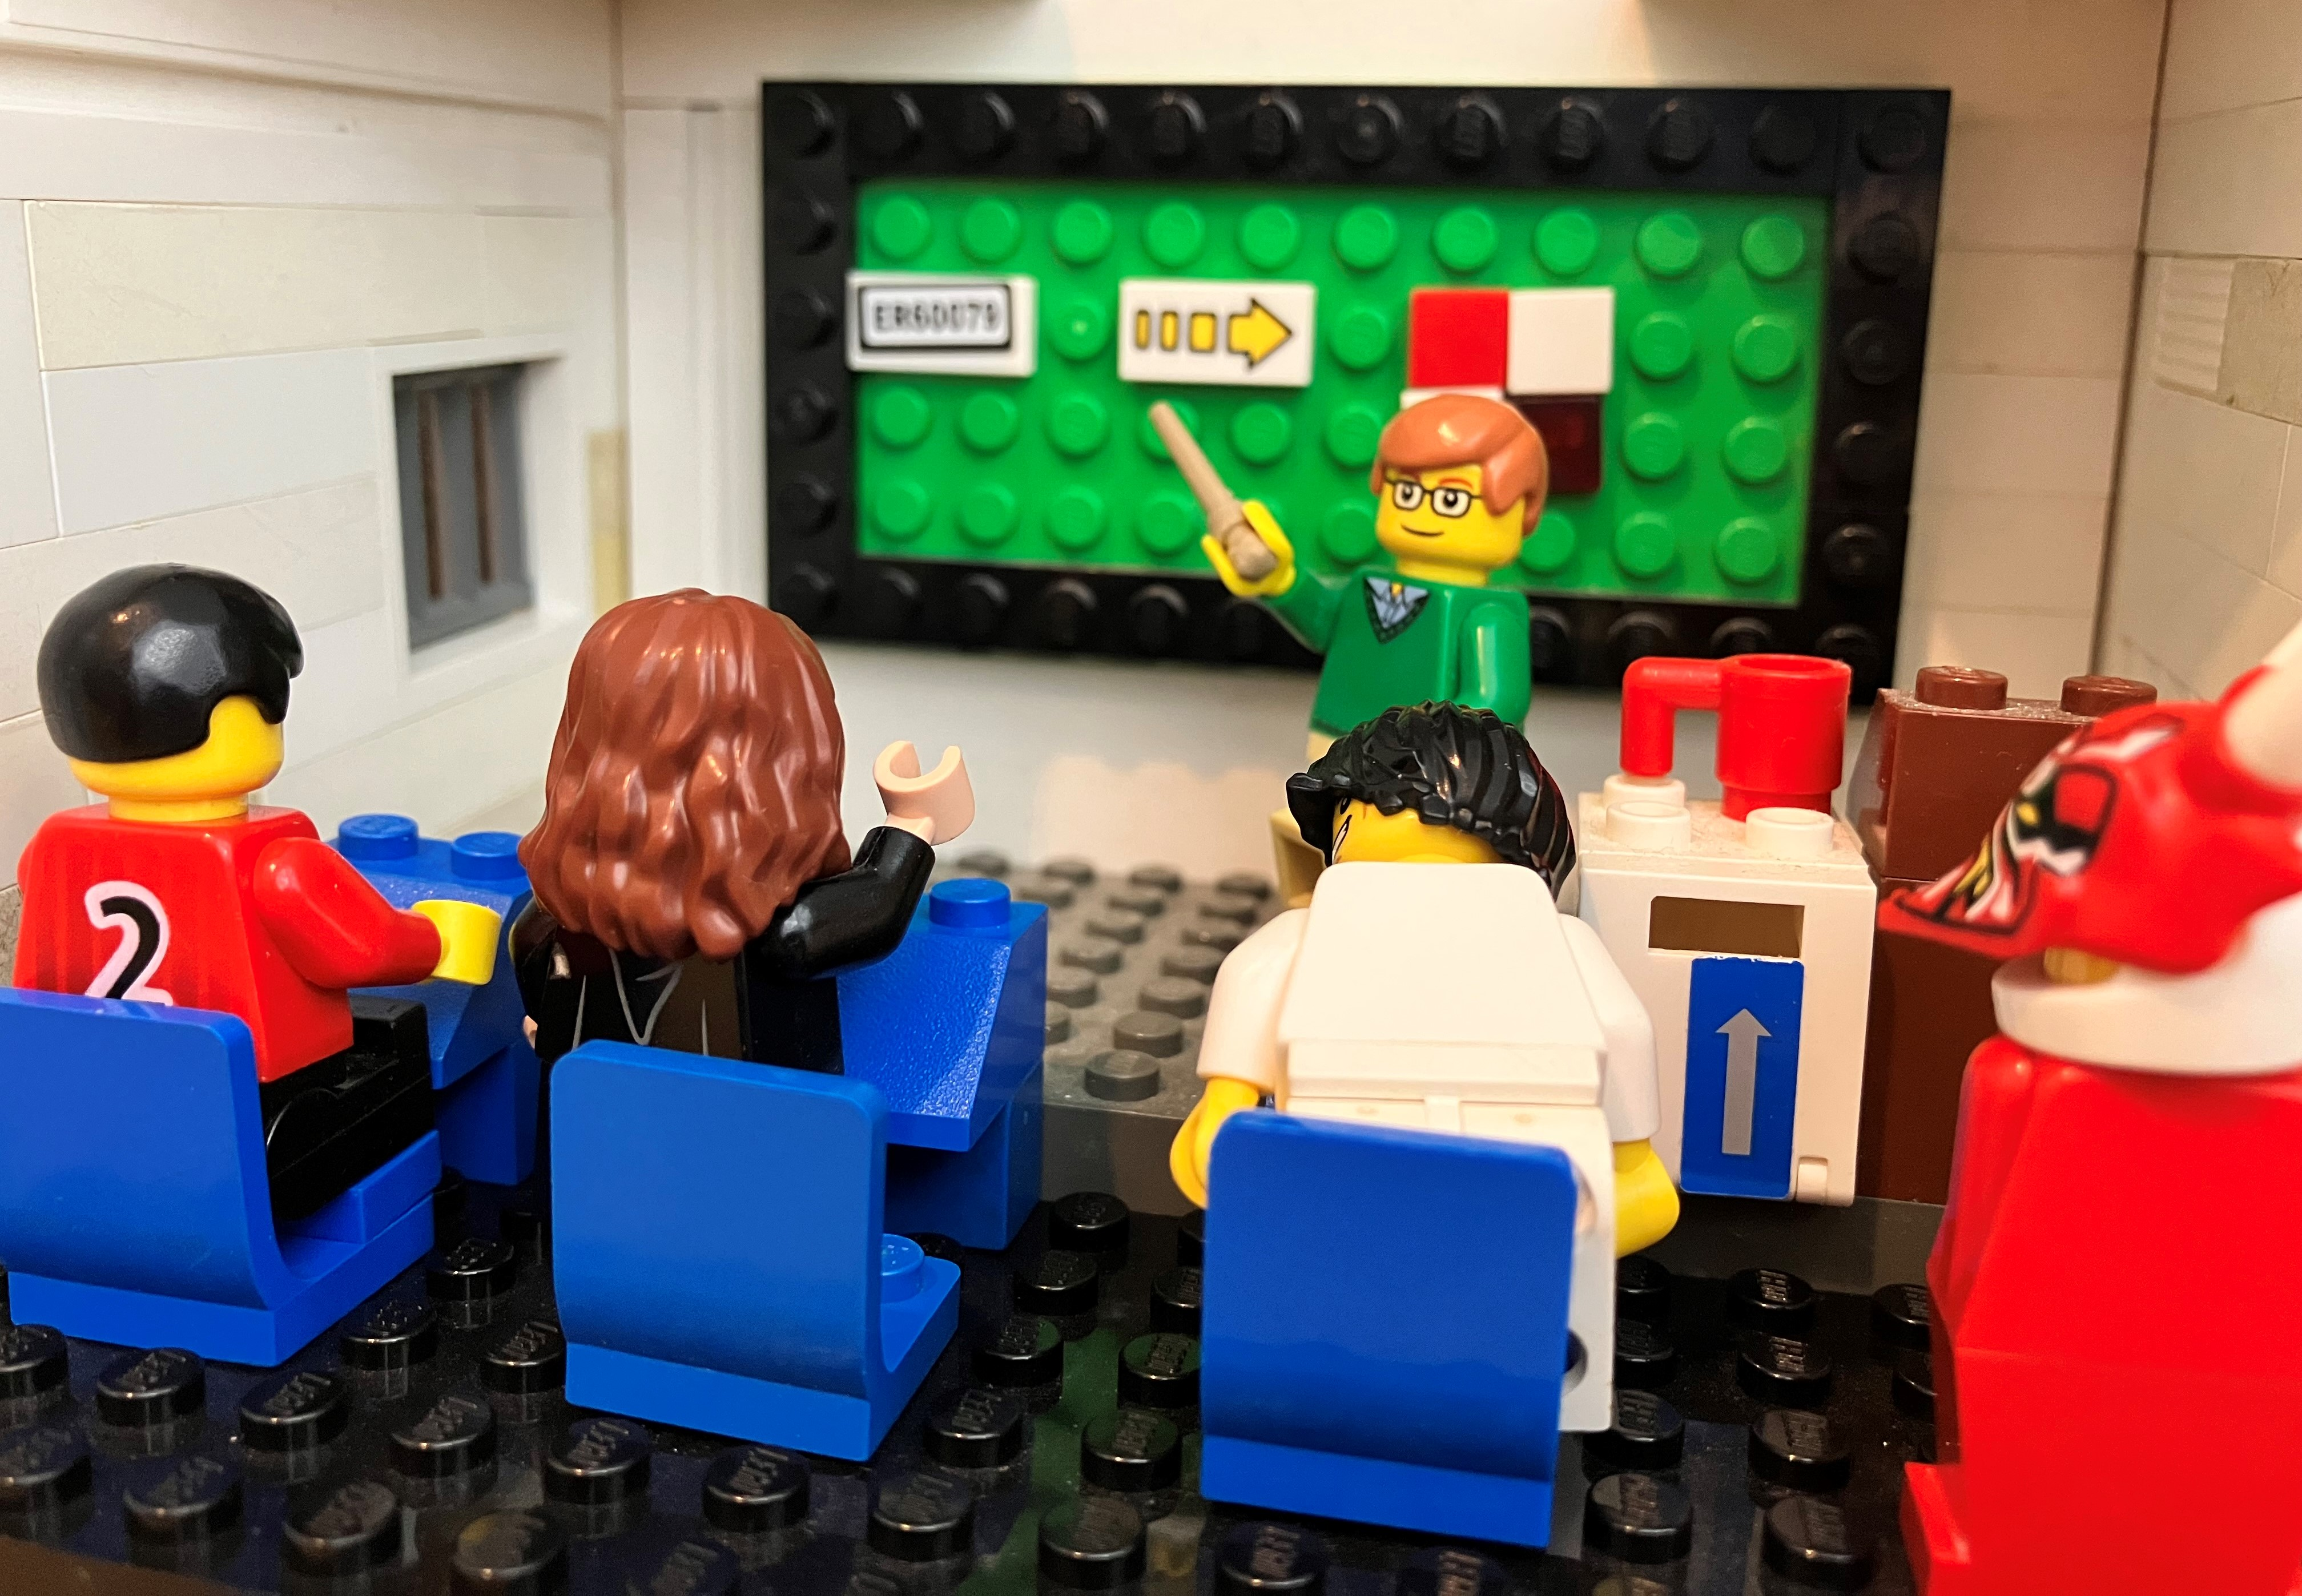
\includegraphics[width=4in]{front/motive.jpg}};
          \node at (0,3in) {
                \begin{tikzpicture}
                      \node[text width=3in,
                            fill=black!10,
                            cloud, 
                            cloud ignores aspect, 
                            minimum width=3in, 
                            minimum height=3in,
                            scale=1.25,
                            draw] at (0,2in) {That's right, this boring bit is really relevant today because it was on my qualifying exam...};
                      \node[text width=3in, scale=1] at (1in,1.5in) {...and on my advisor's exam...};
                      \node[text width=3in, scale=0.75] at (-0.5in,1.25in) {...and his advisor's exam...};
                      \node[text width=3in, scale=0.65,rotate=5] at (0.85in,1in) {...then Bernoulli---or was it his brother?!---homework find out which one...};
                      \node[text width=3in, scale=0.5,rotate=-7] at (-0.75in,0.85in) {...funny story, Archimedes...};
                                  
                \end{tikzpicture}};
    \end{tikzpicture}
\end{center}
\newpage



Algebra today is taught by example. First groups, then rings,
then fields, then modules, then bigger groups, then crazier non-associative
rings, then groups and rings with outside influences like topology, analysis,
and geometry. Today there are few general-practice algebraist.  There are
instead geometric group theorist, algebraic geometers, commutative ring
theorist, representation theorist, non-associative algebraist, computational
algebraist (that's me), and even those topics are too general for any one
theorist to master. Its acceptable because we still know one another and can ask
a specialist when we do not understand. 

The problem is that our algebra textbooks are getting thicker, some split into
multiple volumes. We have not covered an entire text for decades and few  
students can familiarize themselves with the entire book in one year.
One outcome has been to emphasize the good-old-days of successful theory from the
1800's and early 1900's.  Sylow's theorems, Wedderburn-Artin, Hilbert's
Nullstallensatz, Krull-Schmidt, Jordan-H\"older, Frobenius reciprocity. But a
lot a has happened in the century since.  Another approach has been for teachers to
pick their favorites making each course different form the next.  
Too many of us follow trends and fashions for this to be reliable (rebellion of 
a trends is a trend in its own right).

What if algebra were not taught by examples?  What if we taught its
underlying structural methodology and saw examples as reinforcing the theory
not being the theory.  What if instead of proving Krull-Schmidt for modules and
saying ``the same idea applies for groups and rings'', we just proved a theorem
that applied to modules, groups, and rings?  There is no harm in repetition and
useful examples.  I understand why we skip details of homomorphisms of modules
or Lie algebras because by the time students see these, they have seen enough
examples of that concept.  Yet, that behavior goes very wrong very quick.  Ask
your students (ask yourself) What is the kernel of a homomorphism of semigroups?
Monoids?  Homomorphism on $\mathbb{N}$?  Basic as these are, experience 
with groups and rings will not answer these riddles.
When we use our models instead of our theory 
we loose something.  

\begin{center}
    \textbf{Abstract algebra is not abstract enough.}
\end{center}


% \include{front/preface}
% \input{front/timeline}
\cleardoublepage


\tableofcontents
\cleardoublepage

% \input{front/notation}
\cleardoublepage


\mainmatter%%%%%%%%%%%%%%%%%%%%%%%%%%%%%%%%%%%%%%%%%%%%%%%%%%%%%%%


\import{1-intro}{index}

\part{Language of Algebra}
\import{2-grammar}{index}
\import{3-naturals}{index}
\import{4-strings}{index}
\import{5-cfg}{index}
\import{5-free-sub}{index}
\import{6-operators}{index}
\import{7-lambda}{index}
\import{7-reasoning}{index}








\part{Theory of Algebra}

\import{allegory}{index}

\import{9-noether}{index}


\newpage
{\huge Answers...}
\begin{itemize}
      \item[$\Box$] What is an equation? A pair of formulas form the same unambiguous context-free grammar.
      \begin{itemize}
          \item[$\Box$] What is a context-free grammar? A model for expressing complex induction.
  
          \item[$\Box$] What is a variable? An element of the variable alphabet.
  
          \item[$\Box$] What makes an operator-variable? 
          A production rule in a context-free grammar set up as the signature of the formula.
  
          \item[$\Box$] What is a formula? A parse-tree of a context-free grammar with variables.

          
      %     \item[$\Box$] What is equality? (A variable with the Leibniz law as elimination.)
  
      \end{itemize}
\end{itemize}
{\huge Questions...}
\begin{itemize}
      \item[$\Box$] What is an algebra? (A collection of types and operators matched to the 
      production rules of a context-free grammar.)
      \begin{itemize}
          \item[$\Box$] What substitutes for an operator in a formula? 
          (A $\lambda$ which can be typed to match the production rules of the grammar.)
  
          \item[$\Box$] What substitutes for a variable in a formula?
          (Terms of of the types matched to the grammar.)
          
          \item[$\Box$] What substitutes for equality in a formula? 
          (A congruence on the algebra.)
      \end{itemize} 
      
  \end{itemize}





\import{90-algebras}{index}


\part{Appendices}
\appendix


\chapter{Please don't contradict me}

\begin{quote}
    Proof by contradiction is dangerous because 
    when you make a mistake it helps you.
    \hfill J.P.~Serre.
\end{quote}
% \section{Introduction}
We all have argued something is false by considering the consequences 
of assuming it is true.   The idea occurs throughout cultures and 
eras and so it seems sound.  Mathematics has numerous examples including 
the following claims.
\begin{itemize}
    \item $\sqrt{2}$ is irrational.
    \item There are infinitely many primes.
    \item The decimal numbers outnumber the integers.
\end{itemize}
In each of these we argue by assuming the opposite, for example 
that $\sqrt{2}=a/b$, and we work towards a difficulty we cannot accept.
Many authors and speakers of today describe such proofs as 
\emph{indirect}.  Some even say they are \emph{proofs by contradiction}.
The very bold will invoke latin titles
\emph{reducto ad absurdum}, a nod to the rich history.

The latin titles not withstanding, western philosophy actually spent most of the
last 2 millennia concerned with a poetic schemes for reasoning described by
Socrates and known as \emph{syllogisms}.  There are 256 syllogisms, of which 24
are called valid.  Even the form of syllogisms is different from what 
today's authors mean by indirect proof, or proof by contradiction.  Those are
much more recent concepts due in large part to the polymath David Hilbert, who
published a widely read treatise on the foundations of math in 1927.
Contemporaries to Hilbert, namely Brouwer, Heyting, and Kolmogorov (BHK) are far
less known, but their work was almost exclusively on foundations 
which permitted them to notice and craft a far more nuanced ontology of arguments.

Mathematics today is such a broad field with connections to so many areas that
it benefits enormously from the informal and expedient treatment given by
Hilbert's system.  Yet, a growing number of fields including Computer Science
and Linguistics, as well as the mathematical disciplines of Universal Algebra,
Lattices,  Topology, \& Category Theory; are today turning towards the lessons
of his contemporaries.  Arguably the most influential difference is the clarity
that the \emph{BHK interpretation} brings to the study of negatives.

\section{What is a negative?}
In symbolic form a negative is a sentence beginning in negation, 
often written $\neg P$.  In our examples language can serve to 
hide this negation so it is a good practice to begin teasing out 
what is hidden.
\begin{itemize}
    \item It is \emph{not true} that $\sqrt{2}$ is rational.
    \item It is false that the set of primes is finite.
    \item There is no bijection $\mathbb{R}\to \mathbb{Z}$
\end{itemize}
To make this even more stark we can use some symbolic logic.
\begin{itemize}
    \item $P\equiv \sqrt{2}=a/b$.  \textbf{Claim} $\neg P$.
    \item $Q\equiv (\exists n\in \mathbb{N})(|\mathsf{Primes}|=n)$. 
    \textbf{Proposition} $\neg Q$
    \item $R\equiv (\exists f:\mathbb{R}\to \mathbb{Z})(g:\mathbb{Z}\to \mathbb{R})(f\circ g=1)\wedge (g\circ f=1)$.
    \textbf{Theorem} $\neg R$.
\end{itemize}

\subsection*{Choices}
Already you may notice a bit of a predicament.  We seem to have options.  In the
case of primes we appealed to a definition of finite, for instance
\begin{center} 
    ``a set is finite
if it has bijection to a set $\{1,\ldots,n\}$ for some natural number $n\in
\mathbb{N}=\{0,1,\ldots\}$''
\end{center}
We might have wondered instead if we could use a direct definition of 
infinite instead, perhaps Cantor's definition:
\begin{center}
    ``a set with a bijection to a proper subset''.
\end{center}
If we did so then ``There are infinitely many primes'' would cease 
to be a negative.  

Of course if we switch definitions then 
it is on us to also demonstrate that those definitions agree.
There in hides our missing negative.
In our setting, if your approach to proving that there are 
infinitely many primes will somewhere use a phrase like 
\begin{center}
    ``Let $p_1,\ldots,p_n$ be the assumed list of all primes...''
\end{center}
then plainly you are using the first of the two possible definitions 
and your proof is in fact proving a negative.  We shall get to ways to 
prove negatives in a moment but now is a good time to acknowledge our 
problems with the concept.

\section{Psychology of negatives}
``You cannot prove a negative!'' This is a premise often used in arguments both
mindless and seemingly profound.  It is picked up at an early age rooting its
philosophy deep into a our early intuition.  
If it is true we would do well to steer clear of arguments 
that prove negatives and attach different rationalizations to our 
arguments, such as ``proof by contradiction, modus tolens'' and such.
But is this phrase even true?

To begin with the idiom itself is a negative.  It is equivalent to stating:
\begin{center}
    $P\equiv$ ``You can prove a negative''\\
    $\neg P\equiv$ ``You cannot prove a negative.''
\end{center}
So the sentence, if true, would need to be a proof of a
negative, which the sentence argues cannot be done.  So we ought to 
ignore this sentence entirely for logical purposes.

However it is worth acknowledging what this phrase has done 
to readers of proofs.
As psychologist Stephen Law observes in \emph{Psychology Today}, Sept. 15, 2011,
this phrase often adequately summarizes the nature of \emph{doubt}, 
not \emph{truth}.  
As scientists of reason we should like to remove doubt 
and so arguments seen as ``proving a negative'' do indeed deserve 
close scrutiny.


% \subsection*{Negatives arguments read like false arguments.}
One reason for so much doubt in proving negatives is that the arguments lie
adjacent to many known logical fallacies (invalid arguments).  
For instance:
\begin{quote}
    ``I've never seen aliens; so, they do not exist.''
\end{quote}
If we remove the negatives
    ``If aliens exist then I will see them.''
we are often better able to identify our doubts.  Why should I be 
the one to see aliens?

% Mathematicians do not escape these issues in their proofs,
% but they have instead established conventions on the permitted use 
% of these sort of fallacies.  For example, how many proofs can be 
% found that argue with phrases like these:
% \begin{quote} 
%     \emph{It is enough to consider the special case ...}\\
%     \emph{...the argument follows similarly for other cases.}\\
%     \emph{Clearly...}\\
%     \emph{...mutatits mutandis.}
% \end{quote}


% Understanding those contours helps us feel confident in the 
% need for the details of the eventual correct notion.


% \subsection*{Argument from Ignorance}
% Consider the following statements.
% \begin{itemize}
%     \item I don't see aliens so they do not exist.
%     \item No prime less than 100 divides 55,723 so it is prime.
%     % \item It is enough to consider the special case where...
% \end{itemize}
% Hopefully we all recognize these claims are insufficient to be taken 
% as truths, rather, they each merely identify a source for doubt.
% Logicians refer to this  as \emph{Argument from Ignorance},
% the ignorance being the failure to know all the evidence before 
% drawing a conclusion. 

% Mathematics does not escape these concerns, but they do 
% a good job of disguising it to simplify arguments. 
% For instance, many well-intentioned 
% proofs use phrases such as 
% \begin{quote} 
%     \emph{It is enough to consider the special case ...}\\
%     \emph{...the argument follows similarly for other cases.}\\
%     \emph{...mutatits mutandis.}
% \end{quote}
% We can appreciate the expedience that such phrasing permits but 
% it is nevertheless the case that these are attempts to leave out 
% vital evidence by passing judgement on the relative value or ease 
% of acquiring further evidence.  But in truth such arguments appeal to results 
% that the evidence provided cannot validate.  


% Such fallacies are easily remedied into factual claims.
% \begin{itemize}
%     \item I don't see aliens so \emph{I doubt} they exist.
%     \item No prime less than 100 divides 55,723 so \emph{I believe} it is prime.
% \end{itemize}
% In mathematics the expected correction is usually of the form 
% ``Leaving an exercise $X$ to the reader, it then follows ...''.
% Under the principle of assuming good intent we are inclined 
% in most setting to grant the author such implicit alterations
% to their statement.

% \subsection*{Burden of Proof}
% Another family of errors that supports misgivings about ``proving a negative''
% comes from claims like these.
% \begin{itemize}
%     \item Aliens do exist unless you show me why they don't.
%     \item 55,723 is prime until you show me a factor.
% \end{itemize}
% Philosopher's refer to this as \emph{shifting the burden of proof}
% and declare it to be mistake of reasoning.  Proofs in mathematics 
% often do the same ending a brief proof with stock phrases such as 
% \begin{quote}
% \emph{...which leads to a contradiction.}
% \end{quote}
% Once more our read must decide what is being contradicted and how.  It is 
% in every sense a shift of the burden of truth but again one where 
% good will makes its use acceptable.

% % \subsection{Linguistic negatives}
% % Neither \emph{Argument from Ignorance} nor \emph{Burden of Proof} fallacies are
% % unique to negatives.  The fundamental struggle is that when proving a negative
% % we begin precisely doubting what we claim.  So the very language of our argument
% % entertains the vary vocabulary that often leads us to speak forcefully but in
% % error.





% % \subsection{Detecting negatives}

% % \section{Arguing negatives to a machines}
% % Since human language has such a p

% % The actual name is \emph{proving a negative}.

% % Many books introducing scholars to reasoning do not even mention this 
% % type of proof by name.  Some authors even make the effort to credit 
% % historical studies given methods of proofs their latin titles
% % \emph{modus ponens} and \emph{tolens}, and \emph{reducto ad 
% % absurdum}.  Have we lost track of the methods of proofIf it seems  did we come so far and loose track of the method 
% % and name for a proof we use so often?


% Knowing the difference makes certain that our arguments on based 
% on firm reasoning that ends in the desired conclusion.
% Without it we may succeed in an argument that lowers our doubt 
% below what we tolerate but leave open the door that others may 
% still suspect our claims.





\section{Examples.}

\begin{proposition}
   $\sqrt{2}$ is \emph{irrational}. 
\end{proposition}
First we identify the negativity.  Here \emph{ir-}rational is a 
linguistic trick to mean \emph{not} rational.  So we actually mean the following.

\begin{proposition}[Formal Form]
    $\neg(\sqrt{2}\in \mathbb{Q})$
\end{proposition}

Second we identify the context, in this case that means to explain 
some possible meaning of rational.

\begin{definition}
    A \emph{rational number} is a solution to an equation 
    $a=bx$ for integers $a,b$ with $b\neq 0$.
    We write $x\in \mathbb{Q}$.
\end{definition}

So we we break up the proof to see what is happening.
\begin{lemma}\label{lem:irrational}
    If there are integers $a,b$ for which $b\sqrt{2}=a$ then 
    $b=0$.
    % $(\exists a,b\in \mathbb{Z})(b\sqrt{2}=a)\Rightarrow (b=0)$.
\end{lemma}

This lemma is the heart of the proof and can be proved directly.
To focus on the $\sqrt{2}$ it might be best to skip the proof and return 
once we understand the larger claim.

\begin{proof}
    To prove the implication, assume the hypothesis, in this case 
    that for integers $a,b$ $b\sqrt{2}=a$.
    If $b<0$ then replace with $(-a,-b)$.
    So $S=\{b\in \mathbb{N}\mid (\exists a\in \mathbb{Z})(b\sqrt{2}=a)\}$
    is non-empty.  Let $b\in S$ be the least element of $b$, and 
    let $a$ be such that $b\sqrt{2}=a$.
    Square both sides to find $2b^2=a^2$.  So $2|aa$ so by Euclid's 
    Lemma $2|a$. Thus $4|a^2=2b^2$ and so $2|b^2$ which by 
    Euclid's lemma proves $2|b$.  Therefore $(b/2)\sqrt{2}=(a/2)$ 
    so $b/2\in S$.  Since $b$ is minimum $b/2=b$  Therefore 
    $b=0$.  Since $b\neq 0\equiv (b=0\Rightarrow \bot)$ and $b=0$,
    $\bot$ follows.  Therefore $(b\sqrt{2}=a)\Rightarrow \bot$.
    So $\sqrt{2}$ is irrational.
\end{proof}

\begin{proposition}[Formal Form]
    $(\sqrt{2}\notin \mathbb{Q})\equiv (\sqrt{2}\in \mathbb{Q}\Rightarrow \bot)$
\end{proposition}
\begin{proof}
    Assume $\sqrt{2}\in \mathbb{Q}$.  That means that there are 
    integer $a,b$ such that $a=b\sqrt{2}$ and $b\neq 0$.
    Next by Lemma~\ref{lem:irrational} we also know 
    that if $b\sqrt{2}=a$ then $b=0$. 
    Finally $b\neq 0$ means $(b=0)\Rightarrow \bot$, 
    and $b=0$; so, we deduce $\bot$.
    Dismissing the assumed hypothesis we have shown 
    $(\sqrt{2}\in \mathbb{Q})\Rightarrow \bot$.
    That is, $\sqrt{2}\notin \mathbb{Q}$.
\end{proof}

\begin{proposition}
    $(|\mathbb{N}|\neq |\mathbb{R}|)\equiv [(|\mathbb{N}|=|\mathbb{R}|)\Rightarrow \bot]$. 
\end{proposition}

\begin{lemma}\label{lem:diagonal}
    If $f:\mathbb{N}\to \mathbb{R}$ is a function then there is 
    an $x^f\in \mathbb{R}$ such that the $k$-th decimal place of 
    $x^f$ is
    \begin{align*}
        x^f_k & = \left\{\begin{array}{cc}
            f(k)_k+1 & f(k)>0\\
            9 & f(k)=0
        \end{array}
        \right.
    \end{align*}
\end{lemma}

This proof is again the heart of the proposition but it is not a negative, 
though in this case case it does have an embedded negative in premise 
``$x$ is not in the image of $f$''.  However the full sentence reads 
 and so this is not a negative itself.

\begin{proposition}
    $\neg (\exists f:\mathbb{N}\to \mathbb{R})(\forall x\in \mathbb{R})(\exists k\in\mathbb{Z})(f(k)=x)$
\end{proposition}
\begin{proof}
    Assume for there is an $f:\mathbb{N}\to \mathbb{R}$ where 
    for every $x\in\mathbb{R}$ has some $k\in \mathbb{Z}$ such that $f(k)=x$.
    Using the $x^f$ from Lemma~\ref{lem:diagonal} then there is 
    some $k\in \mathbb{Z}$ such that $f(k)=x^f$.  Therefore 
    the $k$-th decimal places of both agree: $f(k)_k = x^f_k$.
    Therefore $f(k)_k=f(k)_k+1$ or $0=f(k)_k=9$.
    In the first case $0=1$ and in the second $0=9$.
    Since $0\neq 1$ and $0\neq 9$ in either case we deduce $\bot$.
    Dismissing the assumption, if there is a surjection $f:\mathbb{N}\twoheadrightarrow \mathbb{R}$
    then $\bot$ follows.  So $\not\exists f:\mathbb{N}\twoheadrightarrow \mathbb{R}$.
\end{proof}



\chapter{Choice without Axioms}

The internet will tell you the axiom of choice says
\begin{quote}
    A cartesian product of non-empty sets is non-empty.
\end{quote}
If this is to be an axiom then it should be something we cannot prove.
Therefore it may come as a shock that this is in fact a theorem even 
in some of the most conservative models of logic such as intuitionisitc 
Martin-L\"of Type Theory.

\begin{theorem}
    Given a type $I$, a function $S:I\to \Type$, and a proposition $P$
    
\end{theorem}


\backmatter%%%%%%%%%%%%%%%%%%%%%%%%%%%%%%%%%%%%%%%%%%%%%%%%%%%%%%%


\bibliographystyle{plain}
% \bibliography{bibliography/tensor_biblio}



\printindex

%%%%%%%%%%%%%%%%%%%%%%%%%%%%%%%%%%%%%%%%%%%%%%%%%%%%%%%%%%%%%%%%%%%%%%

\end{document}





